\documentclass[11pt]{amsart}          
\usepackage[a4paper,verbose]{geometry}
\geometry{top=3cm,bottom=3cm,left=3cm,right=3cm,textheight=595pt}
\setlength{\parskip}{0.3em}
% ==============================
% PACKAGES
% ==============================

\usepackage{amsfonts}
\usepackage{amssymb}  
\usepackage{amsthm} 
\usepackage{amsmath} 
\usepackage{caption}
\usepackage[inline]{enumitem}
\setlist{itemsep=0em, topsep=0em, parsep=0em}
\setlist[enumerate]{label=(\alph*)}
\usepackage{etoolbox}
\usepackage{stmaryrd} 
\usepackage[dvipsnames]{xcolor}
\usepackage[]{hyperref}
\hypersetup{
  colorlinks,
  linkcolor=blue,
  citecolor=blue,
  urlcolor=blue}
\usepackage{graphicx}
\graphicspath{{assets/}}
\usepackage{mathtools}

\usepackage{tikz-cd}
\usepackage{minted}
\usepackage{float}
\usetikzlibrary{
  matrix,
  arrows,
  shapes
}

\setcounter{tocdepth}{1} % Sets depth for table of contents. 

% ======================================
% MACROS
%
% Add your own macros below here
% ======================================

\newcommand{\rr}{{\mathbb{R}}}
\newcommand{\nn}{{\mathbb{N}}}
\newcommand{\iso}{\cong}
\newcommand{\too}{\longrightarrow}
\newcommand{\tto}{\rightrightarrows}
\newcommand{\To}[1]{\xrightarrow{#1}}
\newcommand{\Too}[1]{\To{\;\;#1\;\;}}
\newcommand{\from}{\leftarrow}
\newcommand{\From}[1]{\xleftarrow{#1}}
\newcommand{\Cat}[1]{\mathbf{#1}}
\newcommand{\cat}[1]{\mathcal{#1}}
\newtheorem*{remark}{Remark}
\renewcommand{\ss}{\subseteq}
\newcommand{\hask}[1]{\mintinline{Haskell}{#1}}
\newenvironment{haskell}
  {\VerbatimEnvironment
  	\begin{minted}[escapeinside=??, mathescape=true,frame=single, framesep=5pt, tabsize=1]{Haskell}}
  {\end{minted}}

% ======================================
% FRONT MATTER
% ======================================

\author{Bartosz Milewski}
\title{Initial Coalgebra as a Directed Limit}

\begin{document}

\href{https://github.com/BartoszMilewski/Publications/blob/master/Algebras1.pdf}{Previously}, we talked about the construction of initial algebras. The dual construction is that of terminal coalgebras. Just like an algebra can be used to fold a recursive data structure into a single value, a coalgebra can do the reverse: it lets us build a recursive data structure from a single seed. 

Here's a simple example. We define a tree that stores values in its nodes
\begin{haskell}
data Tree a = Leaf | Node a (Tree a) (Tree a)
\end{haskell}
We can build such a tree from a single list as our seed. We can choose the algorithm in such a way that the tree is ordered in a particular way
\begin{haskell}
split :: Ord a => [a] -> Tree a
split [] = Leaf
split (a : as) = Node a (split l) (split r)
  where (l, r) = partition (<a) as
\end{haskell}
A traversal of this tree will produce a sorted list. We'll get back to this example after working out some theory behind it.

\section{The functor}

The tree in our example can be derived from the functor
\begin{haskell}
data TreeF a x = LeafF | NodeF a x x
\end{haskell}


\begin{haskell}
instance Functor (TreeF a) where
  fmap _ LeafF = LeafF
  fmap f (NodeF a x y) = NodeF a (f x) (f y)
\end{haskell}

Let's simplify the problem and forget about the payload of the tree. We're interested in the functor
\begin{haskell}
data F x = LeafF | NodeF x x
\end{haskell}

Remember that, in the construction of the initial algebra, we were applying consecutive powers of the functor to the initial object. The dual construction of the terminal coalgebra involves applying powers of the functor to the terminal object: the unit type \hask{()} in Haskell, or the singleton set $1$ in $Set$. 
 
 Let's build a few such trees. Here are a some terms generated by the single power of \hask{F}
\begin{haskell}
w1, u1 :: F ()
w1 = LeafF
u1 = NodeF () ()
\end{haskell}

\begin{figure}[H]
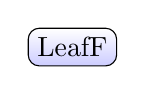
\begin{tikzpicture}[
  baseline=(top.base),
  every node/.style = {shape=rectangle, rounded corners,
    draw, align=center,
    top color=white, bottom color=blue!20}]
  \node (top) {LeafF};
\end{tikzpicture}
\qquad
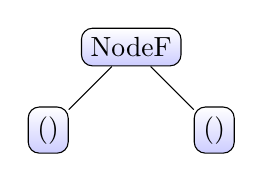
\begin{tikzpicture}[
  baseline=(top.base),
    level distance=3em,
  every node/.style = {shape=rectangle, rounded corners,
    draw, align=center,
    top color=white, bottom color=blue!20}]
    \tikzstyle{level 1}=[sibling distance=6em]
  \node (top) {NodeF}
    child { node {()} }
    child { node {()} };
\end{tikzpicture}
\caption{Trees generated by \hask{F ()}}
\end{figure}

And here are some generated by the square of \hask{F} acting on \hask{()}
\begin{haskell}
w2, u2, t2, s2 :: F (F ())

w2 = LeafF
u2 = NodeF w1 w1
t2 = NodeF w1 u1
s2 = NodeF u1 u1
\end{haskell}
Or, graphically
\begin{figure}[H]
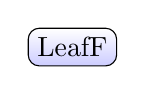
\begin{tikzpicture}[
  baseline=(top.base),
  level distance=3em,
  every node/.style = {shape=rectangle, rounded corners,
    draw, align=center,
    top color=white, bottom color=blue!20}]
  \node (top)  {LeafF};
\end{tikzpicture}
\qquad
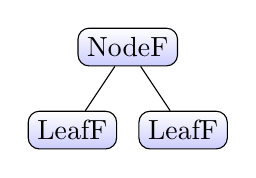
\begin{tikzpicture}[
  baseline=(top.base),
    level distance=3em,
  every node/.style = {shape=rectangle, rounded corners,
    draw, align=center,
    top color=white, bottom color=blue!20}]
    \tikzstyle{level 1}=[sibling distance=4em]
  \node (top)  {NodeF}
    child { node {LeafF} }
    child { node {LeafF} };
\end{tikzpicture}
\qquad
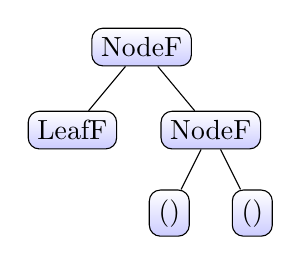
\begin{tikzpicture}[
  baseline=(top.base),
    level distance=3em,
  every node/.style = {shape=rectangle, rounded corners,
    draw, align=center,
    top color=white, bottom color=blue!20}]
    \tikzstyle{level 1}=[sibling distance=5em]
    \tikzstyle{level 2}=[sibling distance=3em]
  \node (top)  {NodeF}
    child { node {LeafF}}
    child { node {NodeF}  
      child { node {$()$} }
      child { node {$()$} }};
\end{tikzpicture}
\qquad
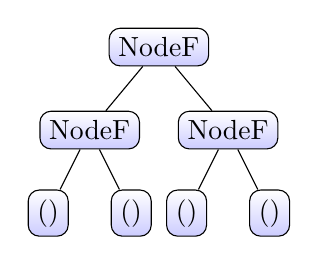
\begin{tikzpicture}[
  baseline=(top.base),
    level distance=3em,
  every node/.style = {shape=rectangle, rounded corners,
    draw, align=center,
    top color=white, bottom color=blue!20}]
    \tikzstyle{level 1}=[sibling distance=5em]
    \tikzstyle{level 2}=[sibling distance=3em]
  \node (top)  {NodeF}
    child { node {NodeF}  
      child { node {$()$} }
      child { node {$()$} }}
    child { node {NodeF}
      child { node {$()$} }
      child { node {$()$} } };
\end{tikzpicture}
\caption{Examples of trees generated by $F^2 1$ or \hask{F (F ())}}
\end{figure}

Notice that we are getting two kinds of trees, ones that have units \hask{()} in their leaves and ones that don't. Units may appear only at the $(n+1)$-st layer (root being the first layer) of $F^n$. 

We are also getting some duplication between different powers of $F$. For instance, we get a single \hask{LeafF} at the $F$ level and another one at the $F^2$ level (in fact, at every consecutive level after that as well). The node with two \hask{LeafF} leaves appears at every level starting with $F^2$, and so on. The trees without unit leaves are the ones we are familiar with---they are the finite trees. The ones with unit leaves are new and, as we will see, they will contribute infinite trees to  the terminal coalgebra . We'll construct the terminal coalgebra as a limit of an $\omega$-chain.

\section{Terminal coalgebra as a limit}

As was the case with initial algebras, we'll construct a chain of powers of $F$, except that we'll start with the terminal rather than the initial object, and we'll use a different morphism to link them together. By definition, there is only one morphism from any object to the terminal object. In category theory, we'll call this morphism $\mbox{!`} \colon a \to 1$ (upside-down exclamation mark) and implement it in Haskell as a polymorphic function
\begin{haskell}
unit :: a -> ()
unit _ = ()
\end{haskell}
First, we'll use $\mbox{!`}$ to connect $F 1$ to $1$, then lift $\mbox{!`}$ to connect $F^2 1$ to $F 1$, and so on, using $F^n \mbox{!`}$ to transform $F^{n + 1} 1$ to $F^n 1$. 

\begin{figure}[H]
\centering
\begin{tikzcd}
  1
  & F 1
  \arrow[l, "\mbox{!`}"]
  & F^2 1
  \arrow[l, "F \mbox{!`}"]
  & F^3 1
  \arrow[l, "F^2 \mbox{!`}"]
  & ...
  \arrow[l, dashed]
\end{tikzcd}
\end{figure}

Let's see how it works in Haskell. Applying \hask{unit} directly to \hask{F ()} turns it into \hask{()}. 

Values of the type \hask{F (F ())} are mapped to values of the type \hask{F ()}
\begin{haskell}
w2' = fmap unit w2
> LeafF
u2' = fmap unit u2
> NodeF () ()
t2' = fmap unit t2
> NodeF () ()
s2' = fmap unit s2
> NodeF () ()
\end{haskell}
and so on.

\begin{figure}[H]
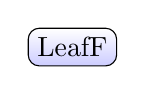
\begin{tikzpicture}[
  baseline=(top.base),
  level distance=3em,
  every node/.style = {shape=rectangle, rounded corners,
    draw, align=center,
    top color=white, bottom color=blue!20}]
  \node (top)  {LeafF};
\end{tikzpicture}
\qquad
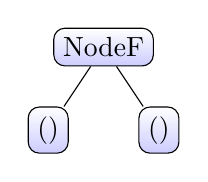
\begin{tikzpicture}[
  baseline=(top.base),
    level distance=3em,
  every node/.style = {shape=rectangle, rounded corners,
    draw, align=center,
    top color=white, bottom color=blue!20}]
    \tikzstyle{level 1}=[sibling distance=4em]
  \node (top)  {NodeF}
    child { node {()} }
    child { node {()} };
\end{tikzpicture}
\qquad
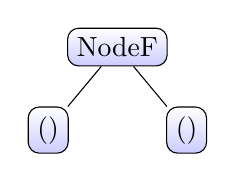
\begin{tikzpicture}[
  baseline=(top.base),
    level distance=3em,
  every node/.style = {shape=rectangle, rounded corners,
    draw, align=center,
    top color=white, bottom color=blue!20}]
    \tikzstyle{level 1}=[sibling distance=5em]
    \tikzstyle{level 2}=[sibling distance=3em]
  \node (top)  {NodeF}
    child { node {()} }
    child { node {()} };
\end{tikzpicture}
\qquad
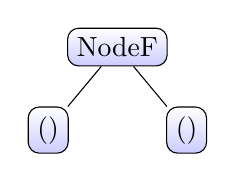
\begin{tikzpicture}[
  baseline=(top.base),
    level distance=3em,
  every node/.style = {shape=rectangle, rounded corners,
    draw, align=center,
    top color=white, bottom color=blue!20}]
    \tikzstyle{level 1}=[sibling distance=5em]
    \tikzstyle{level 2}=[sibling distance=3em]
  \node (top)  {NodeF}
    child { node {()} }
    child { node {()} };
\end{tikzpicture}
\caption{Examples of \hask{fmap unit} acting on trees from the previous figure}
\end{figure}


The following pattern emerges. $F^n 1$ contains trees that end with either leaves (at any level) or values of the unit type (only at the lowest, $(n+1)$-st level). The lifted morphism $F^{n-1}  \mbox{!`}$ (the $(n-1)$st power of \hask{fmap} acting on \hask{unit}) operates strictly on the $n$th level of a tree. It turns leaves and two-unit-nodes into single units \hask{()}.

Alternatively, we can look at the preimages of these mappings---conceptually reversing the arrows. Observe that all trees at the $F^2$ level can be seen as generated from the trees at the $F$ level by replacing every unit \hask{()} with either a leaf \hask{LeafF} or a node \hask{NodeF ()()}. 

\begin{figure}[H]
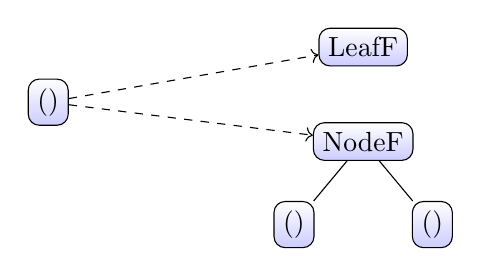
\begin{tikzpicture}[
    level distance=3em,
  every node/.style = {shape=rectangle, rounded corners,
    draw, align=center,
    top color=white, bottom color=blue!20}]
    \tikzstyle{level 1}=[sibling distance=5em]
    \tikzstyle{level 2}=[sibling distance=3em]
    \begin{scope}[shift={(0, 0.5)}]
    \node (A)  {()};
    \end{scope}
    
    \begin{scope}[shift={(4,1.2)}]
        \node (B) {LeafF};
    \end{scope}
    \begin{scope}[shift={(4,0)}]
          \node (C) {NodeF}
               child { node {()} }
               child { node {()} };
    \end{scope}
    \draw [dashed, ->] (A) -- (B);
    \draw [dashed, ->] (A) -- (C);
\end{tikzpicture}
\caption{Universal seed becomes either a leaf or a two-seed-node}
\end{figure}



It's as if a unit were a \emph{universal seed} that can either sprout a leaf or a two-unit-node. We'll see later that this process of growing recursive data structures from seeds corresponds to anamorphisms. Here, the terminal object plays the role of a universal seed that may give rise to two parallel universes. These correspond to the inverse image (a so-called fiber) of the lifted \hask{unit}.

Now that we have an $\omega$-chain, we can define its limit. It's easier to understand a limit in the category of sets. A limit in $Set$ is a set of cones whose apex is the singleton set. 

The simplest example of a limit is a product of sets. In that case, a cone with a singleton at the apex corresponds to a selection of elements, one per set. This agrees with our understanding of a product as a set of tuples. 

A limit of a directed finite chain is just the starting set of the chain (the rightmost object in our pictures). This is because all projections, except for the rightmost one, are determined by commuting triangles. In the example below, $\pi_b$ is determined by $\pi_a$:
\[\pi_b = f_1 \circ \pi_a\]
and so on. Here, every cone from $1$ is fully determined by a function $1 \to a$, and the set of such functions is isomorphic to $a$.
\begin{figure}[H]
\centering
\begin{tikzcd}
  1
  \arrow[d, "\pi_c"]
  \arrow[dr, "\pi_b"]
  \arrow[drr, bend left, "\pi_a"]
  \\
  c
  & b
  \arrow[l, "f_2"]
  & a
  \arrow[l, "f_1"]
\end{tikzcd}
\caption{The limit of this chain is isomorphic to its starting set $a$}
\end{figure}

Things are more interesting when the chain is infinite, and there is no rightmost object---as is the case of our $\omega$-chain. It turns out that the limit of such a chain is the terminal coalgebra for the functor $F$.

\begin{figure}[H]
\centering
\begin{tikzcd}
  1
  \arrow[d, "\pi_1"]
  \arrow[dr, "\pi_{(F 1)}"]
  \arrow[drr, bend left, "\pi_{(F^2 1)}"]
  \\
  1
  & F 1
  \arrow[l, "\mbox{!`}"]
  & F^2 1
  \arrow[l, "F \mbox{!`}"]
  & ...
  \arrow[l, dashed]
\end{tikzcd}
\end{figure}

In this case, the interpretation where we look at preimages of the morphisms in the chain is very helpful. We can view a particular power of $F$ acting on $1$ as a set of trees generated by expanding the universal seeds embedded in the trees from the lower power of $F$. Those trees that had no seeds, only \hask{LeafF} leaves, are just propagated without change. So the limit will definitely contain all these trees. But it will also contain infinite trees. These correspond to cones that select ever growing trees in which there are always some seeds that are replaced with double-seed-nodes rather than \hask{LeafF} leaves.

Compare this with the initial algebra construction which only generated finite trees. The terminal coalgebra for the functor \hask{TreeF} is larger than the initial algebra for the same functor. 

We have also seen a functor whose initial algebra was an empty set
\begin{haskell}
data StreamF a x = ConsF a x
\end{haskell}
This functor has a well-defined non-empty terminal coalgebra. The $n$-th power of \hask{(StreamF a)} acting on \hask{()} consists of lists of \hask{a}s
\begin{haskell}
ConsF a1 (ConsF a2 (... (ConsF an ())...))
\end{haskell}
The lifting of \hask{unit} acting on such a list replaces \hask{(ConsF a ())} with \hask{()} thus shortening the list by one item. Its "inverse" replaces the seed \hask{()} with any value of type \hask{a} (so it's a \textit{multi-valued} inverse, since there are, in general, many values of \hask{a}). The limit is isomorphic to an infinite stream of \hask{a}. In Haskell it can be written as a recursive data structure
\begin{haskell}
data Stream a = ConsF a (Stream a)
\end{haskell}

\section{Anamorphism}

The limit of a diagram is defined as a universal cone. In our case this would be the cone consisting of the object we'll call $\nu F$, or the greatest fixed point of $F$, with a set of projections $\pi_n$

\begin{figure}[H]
\centering
\begin{tikzcd}
  \nu F
  \arrow[d, "\pi_0"]
  \arrow[dr, "\pi_1"]
  \arrow[drr, bend left, "\pi_2"]
  \\
  1
  & F 1
  \arrow[l, "\mbox{!`}"]
  & F^2 1
  \arrow[l, "F \mbox{!`}"]
  & ...
  \arrow[l, dashed]
\end{tikzcd}
\end{figure}
such that any other cone factors through $\nu F$. We want to show that $\nu F$ (if it exists) is a terminal coalgebra. 

First, we have to show that $\nu F$ is indeed a coalgebra, that is, there exists a morphism 
\[k \colon \nu F \to F (\nu F)\]
We can apply $F$ to the whole diagram. If $F$ preserves $\omega$-limits, then we get a universal cone with the apex $F (\nu F)$ and the $\omega$-chain with $F 1$ on the left. But our original object $\nu F$ forms a cone over the same chain (ignoring the projection $\pi_0$). Therefore there must be a unique mapping $k$ from it to $F (\nu F)$.

The coalgebra $(\nu F, k)$ is terminal if there is a unique morphism from any other coalgebra to it. Consider, for instance, a coalgebra $(A, \kappa \colon A \to F A)$. With this coalgebra, we can construct an $\omega$-chain
\begin{figure}[H]
\centering
\begin{tikzcd}
  A
  \arrow[r, "\kappa"]
  & F A
  \arrow[r, "F \kappa"]
  & F^2 A
  \arrow[r, "F^2 \kappa"]
  & F^3 A
  \arrow[r, dashed]
  & ...
\end{tikzcd}
\end{figure}

We can connect the two omega chains using the terminal morphism from $A$ to $1$ and all its liftings

\begin{figure}[H]
\centering
\begin{tikzcd}
  A
  \arrow[d, "\mbox{!`}"]
  \arrow[r, "\kappa"]
  & F A
  \arrow[r, "F \kappa"]
  \arrow[d, "F \mbox{!`}"]
& F^2 A
  \arrow[r, "F^2 \kappa"]
  \arrow[d, "F^2 \mbox{!`}"]
  & F^3 A
  \arrow[r, dashed]
  \arrow[d, "F^3 \mbox{!`}"]
  & ...
  \\
  1
  & F 1
  \arrow[l, "\mbox{!`}"]
  & F^2 1
  \arrow[l, "F \mbox{!`}"]
  & F^3 1
  \arrow[l, "F^2 \mbox{!`}"]
  & ...
  \arrow[l, dashed]
\end{tikzcd}
\end{figure}

Notice that all squares in this diagram commute. The leftmost one commutes because $1$ is the terminal object, therefore the mapping from $A$ to it is unique, so the composite $\mbox{!`} \circ F \mbox{!`} \circ \kappa$ must be the same as $\mbox{!`}$. $A$ is therefore an apex of a cone over our original $\omega$-chain. By universality, there must be a unique morphism from $A$ to the limit of this $\omega$-chain, $\nu F$. This morphism is in fact a coalgebra morphism and is called the \emph{anamorphism}.

\section{Adjunction}
The constructions of initial algebras and terminal coalgebras can be compactly described using adjunctions.

There is an obvious forgetful functor $U$ from the category of $F$-algebras $C^F$ to $C$. This functor just picks the carrier and forgets the structure map. Under certain conditions, the left adjoint free functor $\Phi$ exists
\[C^F ( \Phi x, a) \cong C(x, U a)\]
This adjunction can be evaluated at the initial object (the empty set in $Set$). 
\[C^F ( \Phi 0, a) \cong C(0, U a)\]
This shows that there is a unique algebra morphism---the catamorphism--- from $\Phi 0$ to any algebra $a$. This is because the hom-set $C(0, U a)$ is a singleton for every $a$. Therefore $\Phi 0$ is the initial algebra $\nu F$. 

Conversely, there is a cofree functor $\Psi$
\[C_F(c, \Psi x) \cong C(U c, x)\]
It can be evaluated at a terminal object
\[C_F(c, \Psi 1) \cong C(U c, 1)\]
showing that there is a unique coalgebra morphism---the anamorphism---from any coalgebra $c$ to $\Psi 1$. This shows that $\Psi 1$ is the terminal coalgebra $\nu F$.

\section{Fixed point}

Lambek's lemma works  for both, initial algebras and terminal coalgebras. It states that their structure maps are isomorphisms, therefore their carriers are fixed points of the functor $F$
\[\mu F \cong F (\mu F)\]
\[\nu F \cong F (\nu F)\]
The difference is that $\mu F$ is the least fixed point, and $\nu F$ is the greatest fixed point of $F$. They are, in principle, different. And yet, in a programming language like Haskell, we only have one recursively defined data structure defining the fixed point
\begin{haskell}
newtype Fix f = Fix { unFix :: f (Fix f) }
\end{haskell}
So which one is it? 

We can define both the catamorphisms from-, and anamorphisms to-, the fixed point:

\begin{haskell}
type Algebra f a = f a -> a

cata :: Functor f => Algebra f a -> Fix f -> a
cata alg = alg . fmap (cata alg) . unfix
\end{haskell}

\begin{haskell}
type Coalgebra f a = a -> f a

ana :: Functor f => Coalgebra f a -> a -> Fix f
ana coa = Fix . fmap (ana coa) . coa
\end{haskell}
so it seems like \hask{Fix f}  is both initial as the carrier of an algebra and terminal as the carrier of a coalgebra. But we know that there are elements of $\nu F$ that are not in $\mu F$---namely infinite trees and infinite streams---so the two fixed points are not isomorphic and cannot be both described by the same \hask{Fix f}.

However, they are not unrelated. Because of the Lambek's lemma, the initial algebra $(\mu F, j)$ gives rise to a coalgebra $(\mu F, j^{-1})$, and the terminal coalgebra $(\nu F, k)$ generates an algebra $(\nu F, k^{-1})$. 

Because of universality, there must be a (unique) algebra morphism from the initial algebra $(\mu F, j)$ to  $(\nu F, k^{-1})$, and a unique coalgebra morphism from $(\mu F, j^{-1})$ to the terminal coalgebra $(\nu F, k)$. It turns out that these two are given by the same morphism $f \colon \mu F \to \nu F$ between the carriers. This morphism satisfies the equation
\[k \circ f \circ j = F f\]
which makes it both an algebra and a coalgebra morphism

\begin{figure}[H]
\centering
\begin{tikzcd}
  F (\mu F)
  \arrow[d, "j"]
  \arrow[r, "F f"]
  & F (\nu F)
  \\
  \mu F
  \arrow[r, "f"]
  & \nu F
  \arrow[u, "k"]
\end{tikzcd}
\end{figure}
Furthermore, it can be shown that, in $Set$, $f$ is injective: it embeds $\mu F$ in $\nu F$. This corresponds to our observation that $\nu F$ contains $\mu F$ plus some infinite data structures. 

The question is, can \hask{Fix f} describe infinite data? The answer depends on the nature of the programming language: infinite data structures can only exist in a lazy language. Since Haskell is lazy, \hask{Fix f} corresponds to the \emph{greatest fixed point}. The least fixed point forms a subset of \hask{Fix f} (in fact, one can define a metric in which it's a dense subset).

This is particularly obvious in the case of a functor that has no terminating leaves, like the stream functor.

\begin{haskell}
data StreamF a x = StreamF a x
  deriving Functor
\end{haskell}

We've seen before that the initial algebra for \hask{StreamF a} is empty, essentially because its action on \hask{Void} is uninhabited. It does, however have a terminal coalgebra. And, in Haskell, the fixed point of the stream functor indeed generates infinite streams 

\begin{haskell}
type Stream a = Fix (StreamF a)
\end{haskell}

How do we know that? Because we can construct an infinite stream using an anamorphism. Notice that, unlike in the case of a catamorphism, the recursion in an anamorphism doesn't have to be well founded and, indeed, in the case of a stream, it never terminates. This is why this won't work in an eager language. But it works in Haskell. Here's a coalgebra whose carrier is \hask{Int}
\begin{haskell}
coaInt :: Coalgebra (StreamF Int) Int
coaInt n = StreamF n (n + 1)
\end{haskell}
It generates an infinite stream of natural numbers
\begin{haskell}
ints = ana coaInt 0
\end{haskell}
Of course, in Haskell, the work is not done until we demand some values. Here's the function that extracts the head of the stream:
\begin{haskell}
hd :: Stream a -> a
hd (Fix (StreamF x _)) = x
\end{haskell}
And here's one that advances the stream
\begin{haskell}
tl :: Stream a -> Stream a
tl (Fix (StreamF _ s)) = s
\end{haskell}

\section{Bibliography}
\begin{itemize}
\item Ad\'amek, \href{http://www.tac.mta.ca/tac/volumes/14/8/14-08.pdf}{Introduction to coalgebra}
\item Michael Barr, \href{https://www.sciencedirect.com/science/article/pii/0304397593900766}{Terminal coalgebras for endofunctors on sets}
\end{itemize}
\end{document}
\maketitle{}